\documentclass[11pt]{article}

\usepackage[utf8]{inputenc}
\usepackage[T1]{fontenc}
\usepackage[margin=1in]{geometry}
\usepackage{amsmath,amssymb}
\usepackage{booktabs}
\usepackage{hyperref}
\usepackage{float}
\usepackage{algorithm}
\usepackage{algpseudocode}
\usepackage{graphicx}
\usepackage{xcolor}
\usepackage{microtype}
\usepackage{parskip}
\usepackage[font=small,labelfont=bf]{caption}

\hypersetup{
  colorlinks=true,
  linkcolor=blue!70!black,
  citecolor=blue!70!black,
  urlcolor=blue!70!black,
}

\title{\textbf{Proof-of-Reality: Binding Multimedia Content to Physical\\
Capture through Ledger-Anchored Feedback Paths}}

\author{
  Sungho Kim\\
  KANT Labs\\
  \texttt{sh@kantlabs.com}
}

\date{May 14, 2026}

\begin{document}

\maketitle

\begin{abstract}
Existing approaches to multimedia provenance---device-signing schemes, sensor
fingerprinting, and blockchain timestamping---are engaged in an unwinnable arms
race against generative AI: they provide probabilistic scores, not
deterministic proofs, and adversarial training continuously erodes their
reliability. Faking is \$0; verifying is increasingly expensive. We present
\textbf{Proof-of-Reality (PoR)}, a framework that exits this arms race by cryptographically binding multimedia
content to a live ledger signal that must be physically embedded at capture
time. Pre-synthesis is computationally infeasible because the signal is
unpredictable before the capture moment; real-time synthesis is bounded by a
configurable freshness window~$W$. The mechanism requires
content to embed a time-varying signal sourced from a public distributed
ledger---specifically, a Solana blockhash with an approximately 400\,ms slot
interval---through a physical feedback path (optical, acoustic, or electrical)
that is re-captured by the same device recording the content. Because the
ledger signal is unpredictable before the capture moment, no adversary can
pre-synthesize content containing a valid embedded signal. Combined with an
on-chain receipt anchoring the content hash to a signed ledger transaction,
PoR provides a cryptographic guarantee that requires no AI detector and is
unconditionally robust against pre-synthesis attacks regardless of synthesis
model capability. For real-time synthesis, PoR imposes a time window~$W$
within which the adversary must complete synthesis and submit a receipt; most
current AI models cannot meet this constraint for the constrained task of
embedding a valid QR code as sensor data. We describe a working
implementation using Solana, an Android application, and a
web-based live blockhash watch service, and analyze adversarial scenarios including
pre-synthesis, real-time synthesis, post-synthesis replay, signal replay, and
device compromise.
\end{abstract}

\smallskip
\noindent\textbf{Keywords:} Proof-of-Reality, content provenance, deepfake detection, physical
feedback path, blockchain anchoring, multimedia authentication, liveness
verification

\clearpage
\tableofcontents
\clearpage

% ===========================================================================
\section{Introduction}
% ===========================================================================

Generative AI has achieved photorealistic synthesis of images and video at
near-broadcast quality. By 2026, commercial diffusion models generate
full-resolution video on demand, voice cloning requires seconds of reference
audio, and face-swap pipelines operate in near real time. The downstream
consequences---fabricated political statements, fraudulent insurance claims,
manipulated court evidence, impersonation-based financial fraud---are material
and accelerating.

The standard response has been to
improve forensic detectors. This approach is structurally flawed for three
reasons. First, generative models can be adversarially trained against any
public detector, making the detector obsolete without the defender knowing.
Second, detectors output a probability score, not a binary fact---every
threshold admits false positives and false negatives, and legal or journalistic
use requires certainty. Third, the attacker only needs to succeed once, while the
detector must succeed on every query. The cost of faking reality has reached
effectively \$0; the cost of reliably verifying it via detection is growing
unbounded.

Attention has therefore shifted to \emph{provenance}: establishing
authenticity at the moment of capture, before any adversary can intervene.
We now survey existing approaches and identify the gap each leaves.

\textbf{Provenance metadata standards.} C2PA~\cite{c2pa} defines
cryptographically signed manifests recording capture device, edits, and chain
of custody. It is robust against metadata stripping but does not detect content
synthesized and signed by a compromised signer. Truepic~\cite{truepic} adds a
closed hardware ecosystem but shares the same fundamental limitation: trust is
in the device key, not the capture act.

\textbf{Sensor fingerprinting.} PRNU~\cite{prnu} uses per-sensor pixel
non-uniformity as a device identifier. Effective against naive forgery, but
subsequent work has shown that adversarial PRNU injection is feasible, and
recent diffusion models have demonstrated realistic PRNU imitation; estimation
attacks derive a target sensor's pattern from its public images.

\textbf{Watermarking.} Invisible watermarks embedded at synthesis time
(e.g., C2PA AI-generated content credentials~\cite{watermarking}) detect AI
provenance cooperatively. They assume cooperative producers and are removed by
re-encoding or cropping.

\textbf{Blockchain timestamping.} OriginStamp~\cite{originstamp} and similar
services prove existence-by-time. PoR differs fundamentally: the ledger data is
embedded \emph{in} the content at capture, not applied to the content hash
after the fact.

\textbf{Hardware attestation.} TPM (Trusted Platform Module)-based remote
attestation~\cite{tpm}, Intel SGX (Software Guard Extensions)~\cite{sgx}, and
ARM TrustZone provide cryptographic evidence of device state. They establish
\emph{which device} signed content, not that the device was physically present
at a real-world scene. PoR complements hardware attestation by adding
physical-temporal grounding.

\textbf{Physical unclonable functions (PUFs).} PUFs~\cite{puf} exploit
manufacturing variations for device identification. Like PRNU, they bind
content to a device but do not verify the capture moment or prevent replay of
previously captured content.

\textbf{Liveness detection.} Anti-spoofing systems in face
authentication~\cite{liveness} require a user to respond to an unpredictable
challenge, making replay of pre-recorded sequences detectable. PoR applies the
same unpredictability principle at the content level: the ledger slot value is
the challenge; the embedded signal is the response.

The fundamental gap is that none of these approaches verifies the
\emph{physical act of capture}. A signing device can be tricked, a sensor
fingerprint can be forged, and a timestamp can be applied to synthetic content.
To our knowledge, no prior work closes this gap through a physical
challenge-response mechanism tied to a public ledger.

This paper presents \textbf{Proof-of-Reality (PoR)}, a framework that closes
this gap through a physical challenge-response mechanism tied to a public ledger.


% ===========================================================================
\section{Proof-of-Reality Framework}
\label{sec:por}
% ===========================================================================

\subsection{Capture Protocol}

\begin{enumerate}
  \item \textbf{Ledger Challenge.} The capture device fetches the current
    slot~$S_0$ and blockhash $H_0 = D(S_0)$ from Solana~\cite{solana}.
    $D(t)$ is unpredictable before $t$ (each slot's hash is derived from the
    previous via a verifiable delay function) and publicly verifiable for any
    past $t$.
  \item \textbf{Physical Embedding.} The challenge is encoded as a physical
    signal---optical (QR code on a display), acoustic (ultrasonic), or
    electrical (sensor modulation)---co-located with the scene, ensuring it
    cannot be inserted digitally after capture.
  \item \textbf{Capture.} A display device co-located with the scene shows a
    QR code encoding the current slot~$S_0$ and $H_0 = D(S_0)$. The sensor
    records the scene, producing content $F(C)$ with the signal physically
    embedded in the same frame or audio sample.
  \item \textbf{Content hashing.} The device computes $h_C =
    \mathrm{SHA\text{-}256}(F(C))$. For JPEG images, the hash covers the
    image data region (from the DQT marker to the end-of-image marker) to
    exclude mutable EXIF metadata.
  \item \textbf{On-chain anchoring.} The device constructs a receipt
    \[
      \mathcal{R} = \texttt{kant:v1|slot=}S_0\texttt{|ih=}h_C\texttt{|bh=}H_0\texttt{|sig=}\sigma
    \]
    where $\sigma$ is an Ed25519 signature over $(h_C, H_0)$ by the device's
    keypair. The signed transaction is submitted to Solana via RPC, which
    returns the confirmed landing slot~$S_R$. The device validates
    $S_R - S_0 \leq W$, bounding the freshness window.
    $\mathcal{R}$ is then embedded in the content file (e.g., EXIF
    \texttt{UserComment}) so that the receipt travels with the content.
\end{enumerate}

\subsection{Verification Protocol}
\label{sec:verify}

Given content $C$ with embedded receipt $\mathcal{R}$:

\begin{algorithm}[H]
\caption{PoR Verification}
\label{alg:verify-por}
\begin{algorithmic}[1]
  \State Compute $h'_C = \mathrm{SHA\text{-}256}(F(C))$.
  \State Using $\sigma$ from $\mathcal{R}$, retrieve the on-chain transaction
    confirmed at slot~$S_R$. Verify $h'_C$ matches the hash recorded in the
    transaction.
  \State Decode the QR code visible in the content to extract $S_0$ and $H_0$.
    Verify $H_0$ matches the Solana blockhash for slot~$S_0$.
  \State Verify $S_R - S_0 < W$.
  \State \textbf{PRNU check} (conditional). Verify the sensor noise residual
    of the content matches the registered pattern for the device. Skip if no
    registry is deployed.
  \State Accept if all checks pass; reject otherwise.
\end{algorithmic}
\end{algorithm}

Step~4 is the core PoR check: it confirms the ledger signal was physically
present in the scene at capture time. Step~2 alone reduces to blockchain
timestamping and does not prove physical capture. Step~5 is conditional on
registry availability and strengthens device binding when deployed.

% ===========================================================================
\section{Implementation}
\label{sec:impl}
% ===========================================================================

The reference implementation comprises three components: \textbf{KANTick},
a web-based live blockhash watch that renders the current Solana slot and
blockhash as a QR code; \textbf{KANTist}, an Android application that decodes
the QR, hashes the captured image, signs and submits the on-chain receipt, and
embeds it in EXIF, and submits the signed transaction to Solana via RPC,
receiving the confirmed landing slot~$S_R$ in return. No
special-purpose hardware is required: any smartphone camera and any screen
capable of displaying a QR code are sufficient.

\textbf{Empirical demonstration.} Five photographs were captured using the
KANTist Android application, each with the KANTick QR code visible in frame.
All five receipts were posted on-chain within 4--5 slots of the QR code's slot
($\approx$1.6--2.0\,s after capture), with a mean of 4.4 slots. On-chain slot
values were verified against the Solana ledger via \texttt{getTransaction} RPC
calls and match the EXIF receipt exactly, confirming the correct confirmed landing slot. This confirms that end-to-end
latency---preview-frame capture, DQT hashing, and Solana submission---fits
comfortably within the freshness window~$W$ (Figure~\ref{fig:kantist-captures}).

\subsection{KANTick: Universal Optical Feedback for Still Images}

\begin{figure}[ht]
  \centering
  
\includegraphics[width=0.45\linewidth]{kantick.png}
  \caption{The KANTick live blockhash watch (\url{https://kantick.kantlabs.com}).}
  \label{fig:kantick}
\end{figure}

For still-image capture with any camera, PoR is realized through
\textbf{KANTick}, a web-based live blockhash
watch. KANTick continuously polls the Solana network for the current slot and
blockhash, signs each blockhash with a dedicated Solana keypair, and renders
the result as a QR code displayed in a browser tab. The QR code payload
encodes the slot number and blockhash.

A photographer displays KANTick on any screen (smartphone, laptop, tablet) and
positions it in the scene being photographed. The camera captures both the
real-world scene and the QR code in the same frame, physically embedding the
current blockhash into the image content. A verifier decodes the QR from the
image, verifies the KANTick signature and the on-chain slot record, and
confirms the embedded blockhash matches the Solana ledger at the claimed slot.

\textbf{Planned enhancement: signing oracle mode.}
In the current deployment the QR payload encodes (slot, blockhash) directly.
Because the blockhash is simultaneously visible to anyone monitoring the Solana
network, a well-resourced adversary could in principle start synthesis the
instant a slot opens, using the public blockhash as the embedding target.
A planned server-side enhancement removes this exposure by replacing the
blockhash in the QR with an Ed25519 signature over it:
\[
  \text{QR payload} = \bigl(\,\text{slot},\;
    \sigma = \mathrm{Ed25519.sign}(sk_{\mathrm{kt}},\, H_0)\,\bigr).
\]
The blockhash $H_0$ is \emph{not} transmitted; the QR carries only the slot
number and the server signature.
Verification is: query Solana for $H_0$ at the claimed slot, then check
$\mathrm{Ed25519.verify}(pk_{\mathrm{kt}},\, H_0,\, \sigma) = \mathrm{true}$,
where $pk_{\mathrm{kt}}$ is the publicly announced KANTick service key.

The security property gained is that $\sigma$ is an exclusive capability of
the KANTick server: no party can produce a valid $\sigma$ for slot $S$ before
the server does, because computing $\sigma$ requires the server's private key.
Even though $H_0$ becomes public at the moment slot $S$ opens, the attacker
cannot fabricate a validly signed QR and must wait to observe $\sigma$ from
the server before they can embed it---placing them behind the server by at
least one network round trip.  This converts KANTick from a blockhash relay
into a \emph{signing oracle}: the signed QR is the unpredictable challenge,
not the raw blockhash.

\subsection{Capture Hardware}

Any smartphone camera serves as the capture device; any screen (smartphone,
tablet, or monitor) running KANTick serves as the display device.
KANTist handles live QR decoding, on-device transaction signing, and receipt
embedding. Figure~\ref{fig:kantist-app} shows the KANTist camera viewfinder
with an active KANTick code detected. A PC-based verifier reads the QR from a
photograph and confirms the on-chain record via Solana RPC.

\begin{figure}[H]
  \centering
  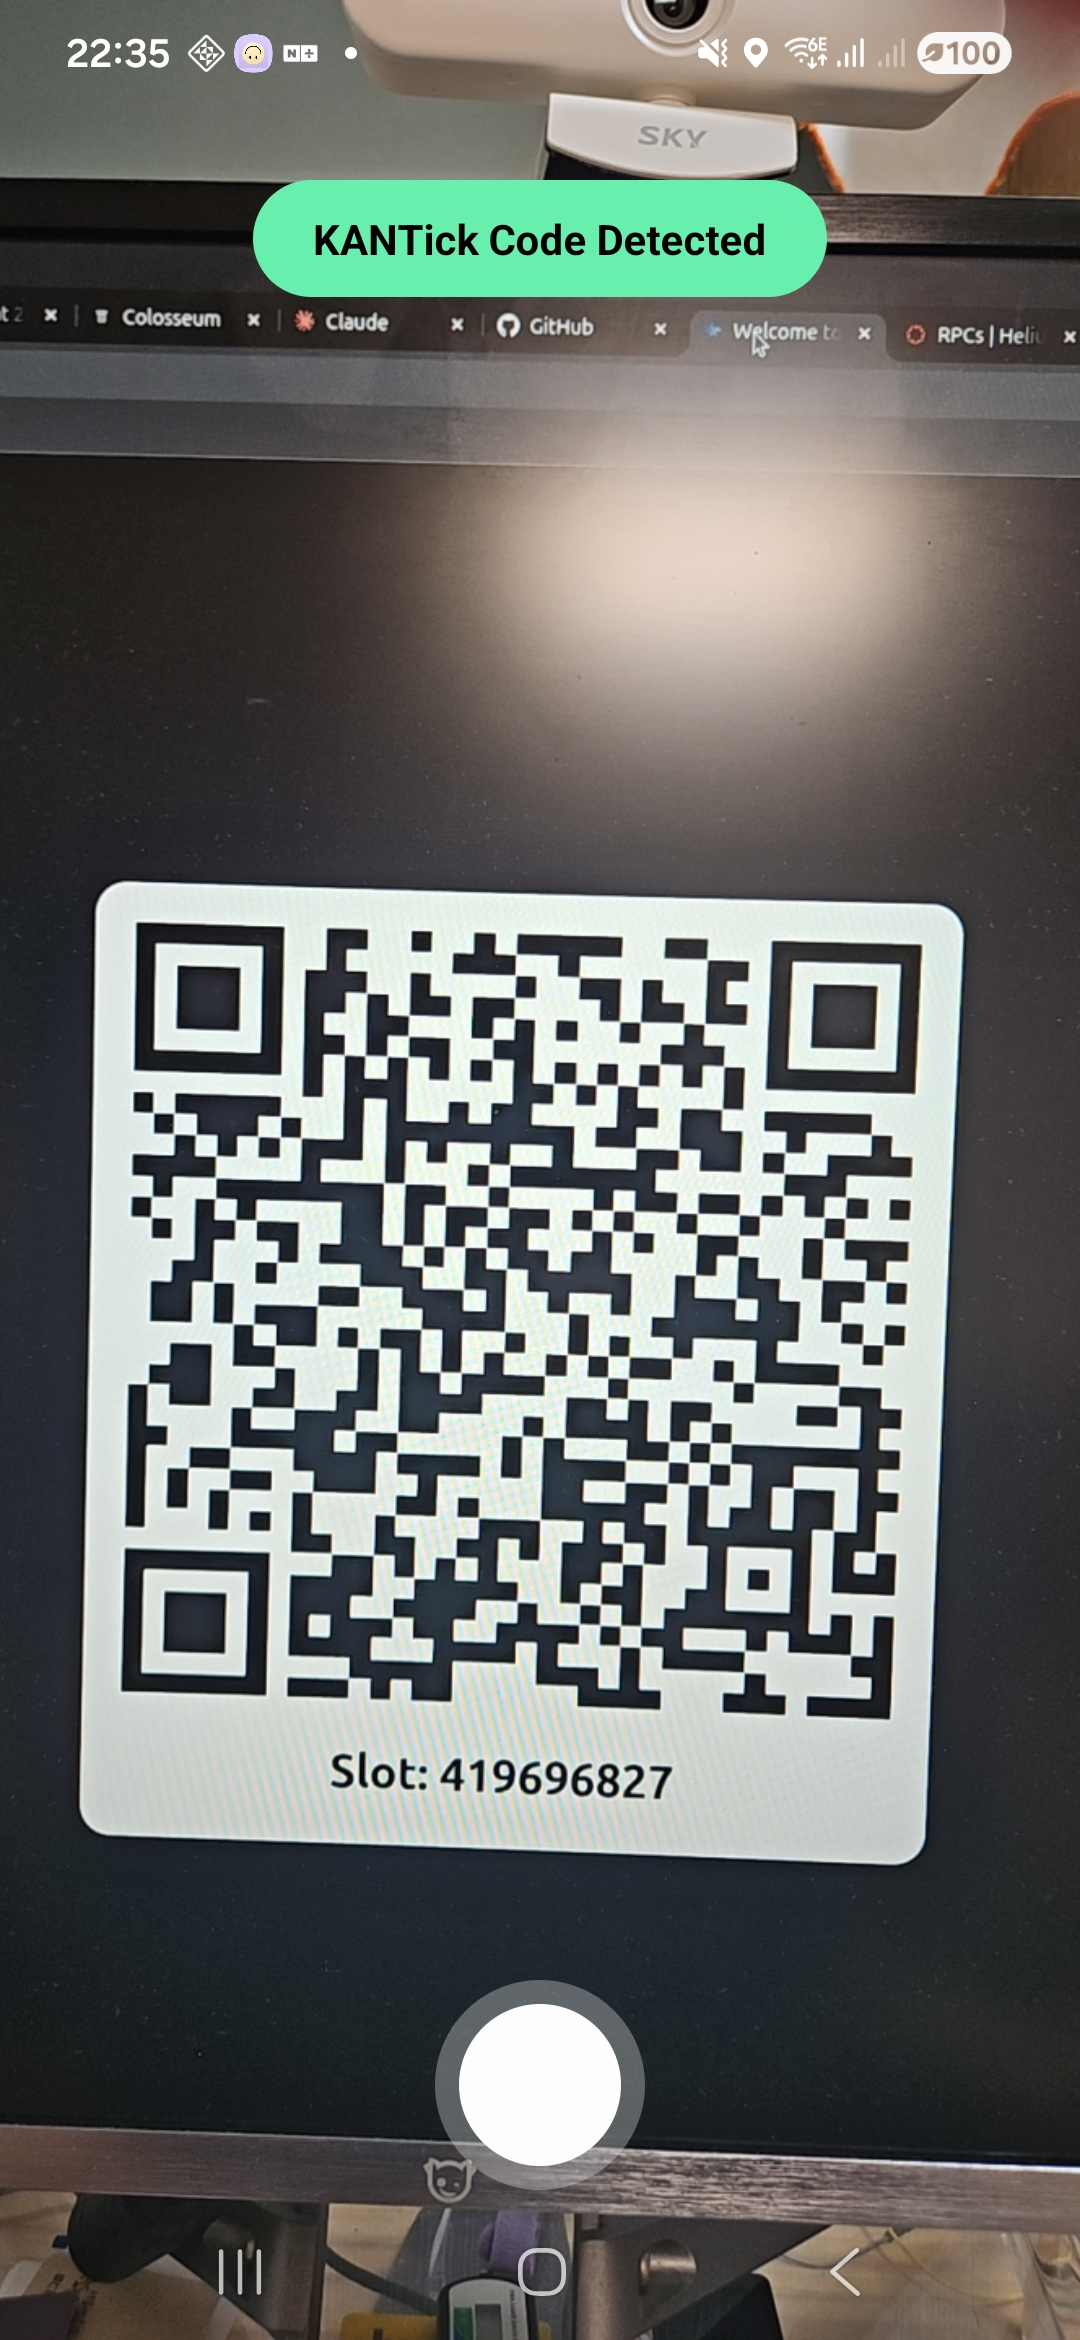
\includegraphics[width=0.38\linewidth]{kantist_app.png}
  \caption{The KANTist Android application: camera viewfinder with the
    ``KANTick Code Detected'' indicator active. Tapping the shutter captures
    the current preview frame, computes the DQT hash natively, signs and
    submits a Solana memo transaction, and embeds the receipt in EXIF\@.}
  \label{fig:kantist-app}
\end{figure}

\subsection{Image Hashing}

The content hash $h_C$ covers the JPEG data from the DQT (Define Quantization
Table) marker to the EOI (End of Image) marker. This range includes all
pixel-level image data while excluding the EXIF/JFIF header, which may be
legitimately modified by camera firmware or photo-management software without
altering pixel content. An adversary modifying any pixel in the compressed
image, or altering the Huffman codes or quantization tables, changes $h_C$ and
breaks the hash check.

\subsection{Blockchain Integration}

The device subscribes to a WebSocket broadcaster service that relays live
Solana slot and blockhash updates from a validator. The broadcaster decouples
the device from direct RPC polling, reducing anchor-acquisition latency and
tolerating intermittent network conditions.

After capture and hashing, the device submits a signed transaction to Solana
via RPC and receives the confirmed slot~$S_R$ and transaction signature.
The device validates $S_R - S_0 \leq W$, where $S_0$ is the slot embedded
in the QR code and $W$ is a configurable freshness window (the reference
implementation uses $W \approx 2{,}000\,\text{ms}$, spanning approximately
five Solana slots). This check prevents an adversary from reusing an old
blockhash against a newly captured image. $W$~is the key security parameter
for the real-time
synthesis defense (Section~\ref{sec:security}). The on-chain transaction
record is publicly auditable: any verifier can query a Solana RPC endpoint
to retrieve $S_R$ and confirm $S_R - S_0 \leq W$ independently, without
relying on any intermediary's assertions.

\textbf{Tightening $W$ via infrastructure.}
The dominant latency contribution in the reference deployment is the
round-trip through a shared public RPC endpoint, which introduces
300--800\,ms of queuing and propagation delay on top of block confirmation.
Running a co-located validator or subscribing to a low-latency RPC service
would reduce this to $\approx$50--150\,ms, shrinking the typical slot delta
to 1--2 slots and allowing $W$ to be tightened to $\approx$2 slots
($\approx$800\,ms). Because $W$ is the primary security parameter against
real-time synthesis (Section~\ref{sec:security}), halving it roughly halves
the synthesis window available to an adversary without any change to the
protocol.

\subsection{Receipt Embedding}

The receipt $\mathcal{R}$ is embedded in the EXIF \texttt{UserComment} tag
(APP1 segment, before the DQT marker). This placement keeps the receipt
outside the hashed region---$h_C$ covers only from the DQT marker onward---so
that embedding the receipt does not invalidate $h_C$. A verifier reads the
\texttt{UserComment} field and then computes $h_C$ from the DQT marker to
confirm integrity.

Both the on-chain anchoring layer and the optical QR embedding layer are fully
operational in the KANTist Android application.

\begin{figure}[ht]
  \centering
  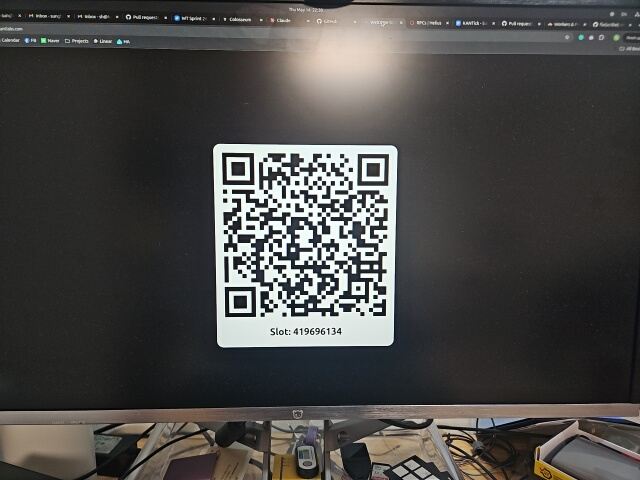
\includegraphics[width=0.55\linewidth]{kantist_capture.jpg}
  \caption{A photograph captured by KANTist with the KANTick QR code in
    frame. The EXIF \texttt{UserComment} receipt records
    \texttt{KANT-qr-slot\,=\,419696134} and
    \texttt{KANT-transaction-slot\,=\,419696138} (slot delta\,=\,4,
    $\approx$1.6\,s). The transaction is publicly auditable at
    \href{https://solscan.io/tx/3xRvtcAQHiDfZz4XdsqocUNf7CbP6yJspeNqgvfsV8VMgxCPKR9kBQm76iGLNZbbJykMtUH6pyTGjc5b5FoVqLpx}{solscan.io}.}
  \label{fig:kantist-captures}
\end{figure}

% ===========================================================================
\section{Security Analysis}
\label{sec:security}
% ===========================================================================

We assume an adversary who can generate photorealistic synthetic content,
can read all public ledger state and has full knowledge of the PoR protocol,
and may purchase and operate a commercial PoR capture device---no aspect of
the system relies on hardware secrecy. The adversary has unbounded offline
compute but bounded real-time synthesis throughput (quantified in
Section~\ref{sec:presynthesis}).

PoR provides \emph{physical capture authenticity}: proof that content was
produced by a real sensor capturing a physical scene, rather than synthesized.
It does not provide \emph{scene truthfulness}: a staged but genuinely
photographed scene yields a valid receipt. We assume the integrity of the
distributed ledger (past blockhashes cannot be rewritten; future blockhashes
are unpredictable) and the soundness of SHA-256 and Ed25519~\cite{nist-sha}.
Scenarios involving physical scene control or device compromise are addressed
in Sections~\ref{sec:device-compromise} and~\ref{sec:discussion}.

\subsection{Pre-Synthesis Attack}
\label{sec:presynthesis}

\textbf{Attack.} The adversary generates synthetic content $C'$ before capture
time~$t_0$, then claims it was captured at~$t_0$.

\textbf{Defense.} The embedded signal must encode $D(t_0) = H_0$, the Solana
blockhash for slot~$S_0$. Because $H_0$ is unpredictable for any time $t' <
t_0$ (Solana's proof-of-history property), the adversary cannot know $H_0$
before $t_0$ and therefore cannot pre-embed a valid signal. Pre-synthesis is
defeated by the unpredictability of~$D(t)$.

\subsection{Real-Time Synthesis Attack}

\textbf{Attack.} The adversary observes $H_0$ the moment it becomes available
at $t_0$, then generates $C'$ in real time embedding~$H_0$, completing before
the freshness window expires.

\textbf{Defense.} A real-time synthesis attack succeeds only if the adversary
can (i)~observe $H_0$ at $t_0$, (ii)~generate photorealistic content with
$H_0$ visibly embedded as a QR code, and (iii)~submit the receipt---all within
the freshness window~$W$.  In the reference implementation,
$W \approx 2{,}000\,\text{ms}$ (Section~\ref{sec:impl}).

The physical feedback path imposes a constraint that synthesis speed alone
cannot overcome.  To pass Tier~2 verification, the adversary must produce an
image in which the correct QR code is present \emph{as sensor data}---not
composited digitally after the fact (digital post-processing changes the image
bytes and fails the hash check, Step~2 of Algorithm~\ref{alg:verify-por}).
The adversary must therefore synthesize a photorealistic scene that
\emph{contains} a specific, structurally valid, decodable QR code encoding the
current blockhash---all within the freshness window~$W \approx 2{,}000\,\text{ms}$.

Standard 20--30-step diffusion pipelines (e.g., SDXL~\cite{sdxl}) require
approximately 1.5--10\,s per full-resolution image on A100/H100 hardware.
More recent models such as FLUX.1~\cite{flux} reduce this to approximately
3--6\,s on H100 with standard inference. Single-step distilled models
(e.g., SANA-Sprint~\cite{sana-sprint}) have reduced \emph{unconstrained}
text-to-image latency to $\approx$0.1\,s on H100---approaching $W$ for raw
inference alone. However, these benchmarks reflect unconstrained generation:
generating a scene that embeds a specific binary QR pattern with exact cell
accuracy is a substantially harder constrained task. Probabilistic diffusion
samplers do not guarantee exact pixel-level structure, and no published
pipeline demonstrates sub-$W$ latency for this constrained setting.
As unconstrained synthesis accelerates toward and below $W$, the constrained-task
gap becomes the primary security margin. Full hardware knowledge of the
PoR device does not relax this constraint: the barrier is not protocol
secrecy but the physics of real-time constrained synthesis. Because $W$ is configurable, it can be tightened (at the cost of
increased rejection of legitimate captures under poor network conditions) to
restore margin as synthesis technology advances.

\subsection{Post-Synthesis Replay Attack}

\textbf{Attack.} The adversary synthesizes content, then waits for a
blockhash~$H'$ that happens to match the signal the adversary wishes to
embed, then submits.

\textbf{Defense.} The freshness check at submission time confirms that the embedded blockhash is
current. The QR payload encodes a specific (slot,
blockhash) pair; an adversary cannot modify the embedded QR after synthesis
without rerunning synthesis from scratch with a different blockhash. Since
future blockhashes are unpredictable (Section~\ref{sec:por}), the adversary
cannot pre-select a convenient blockhash to embed and then wait for it to
appear on the ledger.

\subsection{Signal Replay Attack}

\textbf{Attack.} The adversary photographs a legitimate KANTick QR code
from a previous session and displays it during a synthetic capture, hoping
the verifier accepts the replayed slot and blockhash.

\textbf{Defense.} Each session's QR encodes a specific slot~$S_0$; the
on-chain transaction is confirmed at approximately that slot. A verifier
checks that the on-chain confirmed slot is consistent with the claimed capture
time. Replaying an old QR from session $S_{\mathrm{old}}$ in a new capture
claimed at $S_0 \neq S_{\mathrm{old}}$ causes the slot check to fail.
If the adversary instead claims the original slot time $S_{\mathrm{old}}$,
PoR's cryptographic checks pass; detection then requires external evidence
(contextual timeline, metadata, witnesses) that the claimed time is inconsistent
with observed reality.  PoR's replay defense is therefore scoped to the case
where the adversary claims a \emph{different} time from the replayed session.

\subsection{Device Compromise}
\label{sec:device-compromise}

\textbf{Attack.} An adversary with physical access to the capture device
modifies the firmware to generate and sign fabricated receipts without actually
capturing through the physical feedback path.

\textbf{Defense.} PoR does not assume a tamper-resistant device. The on-chain anchoring layer
is defeated if the device is fully compromised. The optical QR embedding
layer is more robust: a verifier who decodes the QR from the image content
and confirms its slot and blockhash against the on-chain receipt has
evidence that a screen displaying the KANTick watch was physically present in
the scene at capture time. However, an adversary controlling the scene could
place a screen displaying the correct QR in front of a pre-synthesized
background. In the commercial PoR device, manufacturing-time PRNU registration
(Section~\ref{sec:prnu}) substantially raises the attack cost: a compromised
device can be identified by its registered sensor fingerprint, and any
fraudulent content it produces is traceable to its registered owner.

\subsection{Comparison with Hardware Attestation}

\begin{table}[h]
\centering
\caption{Security property comparison.
  \textcolor{green!60!black}{$\checkmark$}~=~satisfied,
  \textcolor{red}{$\times$}~=~not satisfied,
  \textcolor{orange}{$\sim$}~=~partially satisfied or context-dependent.}
\label{tab:comparison}
\begin{tabular}{lccccc}
\toprule
\textbf{Property} & \textbf{C2PA} & \textbf{PRNU} & \textbf{TPM} & \textbf{PUF} & \textbf{PoR} \\
\midrule
Proves capture time             & \textcolor{red}{$\times$} & \textcolor{red}{$\times$} & \textcolor{red}{$\times$} & \textcolor{red}{$\times$} & \textcolor{green!60!black}{$\checkmark$} \\
Proves physical scene presence  & \textcolor{red}{$\times$} & \textcolor{orange}{$\sim$} & \textcolor{red}{$\times$} & \textcolor{red}{$\times$} & \textcolor{green!60!black}{$\checkmark$} \\
Device traceability             & \textcolor{red}{$\times$} & \textcolor{green!60!black}{$\checkmark$} & \textcolor{orange}{$\sim$} & \textcolor{orange}{$\sim$} & \textcolor{green!60!black}{$\checkmark$} \\
No trusted hardware required    & \textcolor{red}{$\times$} & \textcolor{green!60!black}{$\checkmark$} & \textcolor{red}{$\times$} & \textcolor{red}{$\times$} & \textcolor{green!60!black}{$\checkmark$} \\
Resistant to PRNU forgery       & \textcolor{red}{$\times$} & \textcolor{orange}{$\sim$} & \textcolor{red}{$\times$} & \textcolor{red}{$\times$} & \textcolor{green!60!black}{$\checkmark$} \\
Public verifiability            & \textcolor{green!60!black}{$\checkmark$} & \textcolor{green!60!black}{$\checkmark$} & \textcolor{orange}{$\sim$} & \textcolor{red}{$\times$} & \textcolor{green!60!black}{$\checkmark$} \\
Works without network at verify & \textcolor{green!60!black}{$\checkmark$} & \textcolor{green!60!black}{$\checkmark$} & \textcolor{green!60!black}{$\checkmark$} & \textcolor{green!60!black}{$\checkmark$} & \textcolor{red}{$\times$} \\
\bottomrule
\end{tabular}
\end{table}

TPM-based attestation proves \emph{which device} signed content, not that the
device was at a real-world scene at a specific moment. A TPM-equipped device
under adversarial control can sign fabricated content. PUFs identify a device
by its physical characteristics but provide no temporal grounding. PRNU
identifies a sensor but is increasingly forgeable. PoR is the only approach in
the table that simultaneously provides temporal grounding (via ledger
unpredictability) and physical-scene grounding (via the feedback path), without
requiring any trusted hardware component in the device.

The weakness of PoR relative to TPM and C2PA is that verification requires a
live query to a ledger RPC endpoint. The hash and signature checks (Steps~2--3)
can run offline, but they do not constitute PoR verification in isolation: the
critical ledger and blockhash checks (Steps~4--5) require connectivity, and
without them the core temporal guarantee cannot be established.

% ===========================================================================
\section{Discussion}
\label{sec:discussion}
% ===========================================================================

\subsection{Combination with PRNU}
\label{sec:prnu}

PRNU fingerprinting and PoR are complementary: PRNU binds content to a
specific physical sensor; PoR binds content to a specific moment in time and
proves physical capture. In the commercial PoR device, the sensor's PRNU
reference pattern is measured and registered before the unit is sold. The
registry may be hosted on a private manufacturer server or published on a
public ledger, depending on the deployment; in either case, a verifier with
registry access can confirm which specific unit produced an image.

\textbf{Traceability and deterrence.} Because each unit is registered to a
purchaser, any content produced by a PoR device carries an implicit link back
to the buyer. An attacker who purchases a device and uses it to capture a
staged or misleading scene will have their unit identified through PRNU
verification. This does not prevent the attack cryptographically, but it
creates a strong deterrent: fraudulent use of a PoR device is traceable to
the individual who bought it.

\textbf{Combined security.} An adversary who compromises a device's firmware
but not its physical sensor cannot fabricate PoR receipts that also pass PRNU
verification: the fabricated content will not carry the correct sensor noise
pattern. Conversely, an adversary who can replicate a sensor's PRNU cannot
embed valid PoR signals without a live ledger connection at the correct moment.
Defeating the combined system requires simultaneously compromising the firmware
\emph{and} spoofing a device-specific PRNU pattern---a substantially harder
attack than defeating either check alone.

\textbf{Verification step.} Step~7 of Algorithm~\ref{alg:verify-por} requires
querying the PRNU registry for the reference pattern of the device identified
in $\mathcal{R}$ and confirming that the sensor noise residual extracted from
the content matches. A match confirms the specific unit that produced the
image; a mismatch indicates either a compromised device or a forged sensor
fingerprint. Because every commercial PoR unit is registered before sale,
a missing registry entry is itself a verification failure.

\subsection{Limitations}
\label{sec:limitations}

\textbf{Network dependency at capture.} Blockhash acquisition requires connectivity
to the broadcaster service. Connectivity loss immediately before capture can be
partially mitigated by pre-fetching a small number of recent blockhashes while
the connection is live, allowing capture to proceed briefly offline; future
blockhashes cannot be pre-fetched. Note that pre-fetching introduces a
secondary attack surface: if a device caches $k$ blockhashes, an adversary who
has compromised the device can choose among $k$ candidate values offline,
reducing the effective unpredictability of~$H_0$. The pre-fetch window should
therefore be kept as small as operationally necessary.

\textbf{Real-time synthesis frontier.} The security margin against real-time
synthesis is defined by the gap between synthesis latency and the
freshness window. As synthesis accelerates, this margin shrinks. Ongoing
evaluation will quantify the margin as a function of content resolution and
model capability.

\textbf{Continuous video.} This framework addresses single-frame still images.
Extending PoR to continuous video introduces additional challenges---frame-level
deletion and reordering detection, and per-slot transaction cost---that require
a different construction and remain an open problem.

\textbf{Screen relay attack.} An adversary may display a synthesized scene on
a screen that also shows the current KANTick QR code, then photograph the screen
with a legitimate PoR device. The resulting image contains a physically embedded,
valid QR code and passes receipt verification, because the QR was genuinely
re-captured through the optical path. PoR does not inherently distinguish a
real-world scene from a screen displaying a synthesized one. Two complementary
mitigations exist: (i)~\emph{Moiré pattern detection}---cameras photographing
digital displays produce characteristic interference patterns from the
interaction of the screen pixel grid with the sensor grid, which are detectable
algorithmically; and (ii)~\emph{depth sensing}---a co-located depth sensor can confirm that the
scene has physical three-dimensional extent rather than a flat display surface;
viable approaches include ToF (Time of Flight), structured light, and stereo
vision from dual camera lenses, the last of which is available on most modern
smartphones without additional hardware. Neither mitigation is yet integrated
into the reference implementation and both remain directions for future work.

% ===========================================================================
\section{Conclusion}
% ===========================================================================

We have presented Proof-of-Reality, a framework that closes the fundamental gap
in existing multimedia provenance: verifying the physical act of capture rather
than the identity of the signing device. By requiring content to embed a
time-varying, ledger-sourced signal through a physical feedback path during
capture, PoR makes pre-synthesis and post-synthesis replay cryptographically
infeasible without physical presence at the capture scene and moment. A working implementation runs on commodity hardware---any smartphone and a
PC---with no special-purpose devices required. Extension to continuous video remains an open problem. Against pre-synthesis attacks the guarantee is unconditional regardless of synthesis capability; against real-time synthesis it holds as long as the constrained-task synthesis gap persists, and can be maintained by tightening~$W$ as synthesis technology advances.

% ===========================================================================
\section*{Patent Disclosure}
% ===========================================================================

This work is the subject of the following Korean patent applications filed with
the Korean Intellectual Property Office (KIPO):

\begin{itemize}
  \item KR 10-2026-0023748 (Proof-of-Reality framework, filed 2026-02-05).
  \item KR 10-2026-0072171 (full application, filed 2026-04-21).
\end{itemize}

International filings under the Patent Cooperation Treaty are anticipated within
the priority window.

% ===========================================================================
\section*{Acknowledgments}
% ===========================================================================

The author is deeply grateful to Professor Keh-Kuan Sun (Fairfield University)
for invaluable guidance and support in writing this paper.
The author also thanks Gil Se-young (YNP IP) for patent prosecution work.

% ===========================================================================
\bibliographystyle{plain}
\begin{thebibliography}{99}

\bibitem{c2pa}
Coalition for Content Provenance and Authenticity.
\newblock C2PA Technical Specification, v1.4, 2024.
\newblock \url{https://c2pa.org/specifications/}

\bibitem{truepic}
Truepic.
\newblock Truepic Vision: Verified Content for the Enterprise.
\newblock White paper, 2023.

\bibitem{prnu}
J.~Lukas, J.~Fridrich, and M.~Goljan.
\newblock Digital camera identification from sensor pattern noise.
\newblock \emph{IEEE Transactions on Information Forensics and Security},
  1(2):205--214, 2006.

\bibitem{originstamp}
T.~Hepp, P.~Wortner, A.~Schönhals, and B.~Gipp.
\newblock Securing physical assets on the blockchain: linking a novel object
  identification concept with distributed ledgers.
\newblock In \emph{Proceedings of the 1st Workshop on Cryptocurrencies and
  Blockchains for Distributed Systems}, 2018.

\bibitem{watermarking}
I.~J.~Cox, M.~L.~Miller, J.~A.~Bloom, J.~Fridrich, and T.~Kalker.
\newblock \emph{Digital Watermarking and Steganography}, 2nd ed.
\newblock Morgan Kaufmann, 2007.

\bibitem{tpm}
Trusted Computing Group.
\newblock TPM Main Specification, Family 2.0, Level 00, Revision 01.59, 2019.
\newblock \url{https://trustedcomputinggroup.org/}

\bibitem{sgx}
V.~Costan and S.~Devadas.
\newblock Intel SGX explained.
\newblock Cryptology ePrint Archive, Report 2016/086, 2016.

\bibitem{puf}
R.~Pappu, B.~Recht, J.~Taylor, and N.~Gershenfeld.
\newblock Physical one-way functions.
\newblock \emph{Science}, 297(5589):2026--2030, 2002.

\bibitem{liveness}
J.~Galbally, S.~Marcel, and J.~Fierrez.
\newblock Biometric antispoofing methods: A survey in face recognition.
\newblock \emph{IEEE Access}, 2:1530--1552, 2014.

\bibitem{nist-sha}
National Institute of Standards and Technology.
\newblock Secure Hash Standard (SHS).
\newblock FIPS Publication 180-4, 2015.

\bibitem{solana}
A.~Yakovenko.
\newblock Solana: A new architecture for a high performance blockchain.
\newblock Whitepaper, 2018.
\newblock \url{https://solana.com/solana-whitepaper.pdf}

\bibitem{flux}
Black Forest Labs.
\newblock {FLUX.1}: A family of flow-based generative models for text-to-image
  synthesis.
\newblock Technical report, 2024.
\newblock \url{https://blackforestlabs.ai/}

\bibitem{sdxl}
D.~Podell, Z.~English, K.~Lacey, A.~Blattmann, T.~Dockhorn, J.~M\"{u}ller,
  J.~Penna, and R.~Rombach.
\newblock {SDXL}: Improving latent diffusion models for high-resolution image
  synthesis.
\newblock In \emph{International Conference on Learning Representations
  (ICLR)}, 2024.

\bibitem{sana-sprint}
J.~Chen, J.~Yu, Y.~Ge, L.~Yao, E.~Xie, Y.~Wu, Z.~Wang, P.~Ping, et~al.
\newblock {SANA-Sprint}: One-step diffusion with continuous-time consistency
  distillation.
\newblock In \emph{Proceedings of the IEEE/CVF International Conference on
  Computer Vision (ICCV)}, 2025.

\end{thebibliography}

\end{document}
